\documentclass{article}
\usepackage[utf8]{inputenc}

\title{London Calling}
\author{Artur Cassimiro Alves}
\date{April 2019}

\usepackage{natbib}
\usepackage{graphicx}

\begin{document}

\maketitle

\section{Introdução}
London Calling é o terceiro álbum da banda inglesa The Clash lançado em dezembro de 1979. O álbum mistura influências de diversos gêneros musicais como o reggae, o blues e o rock para criar um som punk único.
\cite{wikipediaLondonCalling}

\begin{figure}[h!]
\centering
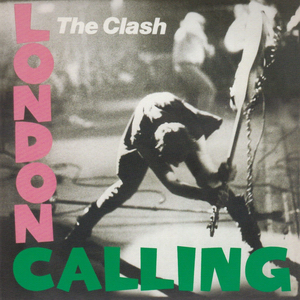
\includegraphics[scale=1.0]{LondonCalling}
\caption{Capa original do álbum}
\label{fig:London Calling}
\end{figure}

\section{Pontos Positivos}
O álbum possui sons extremamente variados e letras surpreendentemente boas, coloridas com a contra-cultura e angústia do movimento punk do Reino Unido.

\section{Pontos Negativos}
O álbum é bem longo e se seus gostos não se alinhem com ele você pode acabar não gostando. (sei lá)

\section{Comparado notas com outras obras de maneira completamente arbitrária}
\begin{table}[h]
\begin{tabular}{|l|l|l|l|l|}
\hline
\textbf{}         & \textbf{London Calling} & \textbf{Let It Be} & \textbf{Philosophy of the World} & \textbf{Psicoacústica} \\ \hline
Técnica           & 8/10                    & 9/10               & -20/10                           & 9/10                   \\ \hline
Conceito          & 10/10                   & 6/10               & 99999/10                         & 9/10                   \\ \hline
Amor \textless{}3 & \textless{}3            & \textless{}3       & \textless{}3                     & \textless{}3           \\ \hline
\end{tabular}
\end{table}

\bibliographystyle{plain}
\bibliography{references}
\end{document}
